\makeatletter
\def\input@path{{../styles/}{../../styles/}{../../../styles/}{../}{../../}{../../../}}
\makeatother
\documentclass{ee102_notes}
% macros.tex - Course meta information
\renewcommand{\course}{EE 102}
\renewcommand{\coursetitle}{Signal Processing and Linear Systems}
\renewcommand{\instructor}{Ayush Pandey}
\renewcommand{\semester}{Fall}
\renewcommand{\year}{2025}
\renewcommand{\shorttitle}{Week 1: Introduction to Signals}
% Use \renewcommand to avoid 'already defined' errors

% The following packages can be found on http:\\www.ctan.org
% \usepackage{graphics} % for pdf, bitmapped graphics files
%\usepackage{epsfig} % for postscript graphics files
%\usepackage{mathptmx} % assumes new font selection scheme installed
%\usepackage{times} % assumes new font selection scheme installed
\usepackage{amsmath} % assumes amsmath package installed
\usepackage{amssymb,mathtools}  % assumes amsmath package installed
\usepackage{xcolor}
\usepackage{pgfplots,subcaption}
\usepackage[hidelinks]{hyperref}
\usepackage{verbatim}
\usepackage{graphicx}
\usepackage{listings}

% -------- listings (Python) ----------
\lstdefinestyle{py}{
  language=Python,
  basicstyle=\ttfamily\small,
  keywordstyle=\color{blue!60!black}\bfseries,
  commentstyle=\color{green!40!black},
  stringstyle=\color{orange!60!black},
  showstringspaces=false,
  columns=fullflexible,
  frame=single,
  framerule=0.3pt,
  numbers=left,
  numberstyle=\tiny,
  xleftmargin=1em,
  tabsize=2,
  breaklines=true,
}
\usepackage[american]{circuitikz}
\usepackage{tikz}
\usepackage{caption}    
\usepackage{lscape}
\usepackage{soul}
\usepackage{tikz}
\usetikzlibrary{calc,angles,quotes,arrows.meta}

\usepackage{hyperref}
\hypersetup{
    colorlinks=true,
    linkcolor=blue,
    filecolor=magenta,      
    urlcolor=blue,
    pdftitle={week1_notes},
    pdfpagemode=FullScreen,
}
%\usepackage{float} 

%\usepackage[demo]{graphicx}
\pgfplotsset{compat=1.18}
% \usepgfplotslibrary{fillbetween}

\newsavebox{\measurebox}

\let\proof\relax\let\endproof\relax


\newcommand{\norm}[1]{\left\lVert#1\right\rVert}
\def\abs#1{\left\lvert#1\right\rvert}
\let\proof\relax
\let\endproof\relax
\usepackage{amsthm}
\usepackage{accents}
\usepackage{relsize}
\newcommand{\ubar}[1]{\underaccent{\bar}{#1}}
\newtheorem{theorem}{Theorem}
\newtheorem{corollary}{Corollary}[theorem]
\newtheorem{lemma}{Lemma}
\newtheorem{proposition}{Proposition}
\newtheorem{statement}{Statement}

\theoremstyle{definition}
\newtheorem{definition}{Definition}
 
\theoremstyle{remark}
\newtheorem*{remark}{Remark}
\theoremstyle{remark}
\newtheorem*{claim}{Claim}
\setlength{\parindent}{0cm}
\newenvironment{nalign}{
    \begin{equation}
    \begin{aligned}
}{
    \end{aligned}
    \end{equation}
    \ignorespacesafterend
}

\renewcommand{\releasedate}{September 3, 2025}
\begin{document}

\section*{EE 102 Week 1, Lecture 1 (Fall 2025)}
\subsection*{Instructor: \instructor}
\subsection*{Date: \releasedate}
\section{Goals}
\begin{itemize}
  \item Introduction to signals: continuous-time and discrete-time
  \item Basic properties of signals: scaling, offset, linearity, and time invariance, and more
  \item Quantifying the energy and power of signals
\end{itemize}

\section{What are signals?}
A \emph{signal} is a set of data or information. This is intentionally defined in a very broad manner. A simple way to understand signals: all mathematical functions that you have studied in your calculus classes are signals if you can attach a physical meaning to the function. Note that a signal need not be a function of time. It is often intuitive to think about functions of time and physical signals are functions of time (often, but not always!).

A \emph{system} maps (that is, it processes) input signals into output signals. So, systems are characterized by their input-output relationships. See Figure~\ref{fig:system} for a visual representation of signals and systems.
\begin{figure}[h]
  \centering
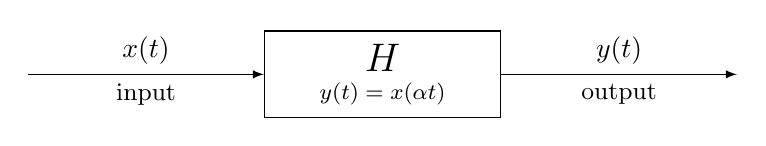
\begin{tikzpicture}[>=latex]
  \node[draw, minimum width=3cm, minimum height=1.1cm, align=center] (H) {\Large $H$\\[-2pt]\footnotesize $y(t)=x(\alpha t)$};
  \draw[->] (-4.5,0) -- (H.west) node[midway, above] {$x(t)$} node[midway, below] {\small input};
  \draw[->] (H.east) -- (4.5,0) node[midway, above] {$y(t)$} node[midway, below] {\small output};
\end{tikzpicture} 
 \caption{A system $H$ that maps input signal $x(t)$ to output signal $y(t)$.}
  \label{fig:system}
\end{figure}

\subsection{Continuous-time and discrete-time signals}
Continuous-time domain is $\mathbb{R}$, and we write continuous-time signals as $x(t)$, if they are continuous functions of time (recall: continuous functions from your math classes). On the other hand, discrete-time domain is $\mathbb{Z}$, and a discrete-time signal is written as $x[n]$, where $n \in \mathbb{Z}$. This means that discrete-time signals are defined only at integer time indices.
\subsection{Sketching signals}
To sketch, draw and label axes, mark key values (peaks, zeros, discontinuities), and indicate any symmetry, periodicity, decay/growth, or piecewise structure (try to identify as many properties as you can before starting to sketch). The best way to start your sketch is to compute the values of the signal at ``easy'' points like, zero, the max time, etc.  

\section{Properties of signals}
\subsection{Scaling}
Time scaling changes the horizontal axis by a constant $\alpha$:
\[
x_s(t)=x(\alpha t).
\]
If $0<\alpha<1$, the signal expands in time whereas if $\alpha>1$, it compresses the signal in time.

\subsection{Offset}
Time shifting offsets the horizontal axis by a constant $T$.  A (right) delay of $T$ seconds is defined by
\[
x_d(t)=x(t-T).
\]
Equivalently, $x_d(t_1+T)=x(t_1)$ for every $t_1$.

\subsection{Linearity of systems}
A system $H$ is \emph{linear} if it satisfies additivity and homogeneity:
\[
H\{x_1+x_2\}=H\{x_1\}+H\{x_2\},\qquad H\{k\,x\}=k\,H\{x\}\quad(\forall k\in\mathbb{C}).
\]
\textit{Example:} the exponential-weighting system $y(t)=e^{-a t}x(t)$ is linear since
\[
H\{x_1+x_2\}=e^{-a t}(x_1+x_2)=e^{-a t}x_1+e^{-a t}x_2=H\{x_1\}+H\{x_2\}.
\]
\textbf{Remark.} ``Linear system'' is a property of the \emph{mapping}, not of the input/output signals. You should not confuse it with a straight-line graph of a scalar function, which you are used to thinking about when thinking about ''linearity''.

\subsection{Time invariance of systems}
A system $H$ is \emph{time invariant} if delaying the input by $T$ produces the same delay at the output:
\[
\text{If }y(t)=H\{x\}(t),\ \text{ then }H\{x(t-T)\}=y(t-T),\quad\forall T\in\mathbb{R}.
\]
Intuition: If your opinion of a friend is dependent on the input about the friend, let's say that input is $x(t)$ (the friend descriptor signal), and seeing that input, you decide your opinion of your friend with an opinion signal called $y(t)$. Then, if your opinion about your friend does not change with time, that is, if you have the same opinion about your friend in the morning, in the evening (and even as the day changes), then your ``opinion-defining'' system (the one that outputs $y(t)$) is time-invariant! However, if your opinion of your friend keeps changing based on the time that you're meeting your friend, then you have a time-varying system of opinion generation (probably not a good trait!). Note that for time-invariant systems, the output is the ``same response'' delivered at the new time. It should not become, e.g., $k\,y(t)$ or $k\,y(t-T)$ depending on $T$.

\subsection{A special signal --- the unit step function}
A unit step function is defined as
\[
u(t) = \begin{cases}
0, & t < 0 \\
1, & t \geq 0
\end{cases}
\]

It is a special signal because it models the ''start'' of something, or an ''onset'' of an event, or more simply, a ''switching on'' of a process. You can shift the time to $t - T$ to delay the start by $T$ seconds, so it's a very versatile signal. Therefore, the unit step function finds use in various applications. 

\textit{Quick check (in-class):} Is the \emph{unit step} $u(t)$ time-invariant? (Trick question: time invariance is a \emph{system} property, not a signal property.)

\section{Energy and power of signals}
We quantify the ``size'' of signals using energy and (time-averaged) power.
For continuous-time signals, we define
\[
E_{\infty} \triangleq \int_{-\infty}^{+\infty}\! |x(t)|^{2}\,dt,\qquad
P_{\infty} \triangleq \lim_{T\to\infty} \frac{1}{2T}\int_{-T}^{T}\! |x(t)|^{2}\,dt.
\]
For discrete-time signals:
\[
E_{\infty} \triangleq \sum_{n=-\infty}^{+\infty} |x[n]|^{2},\qquad
P_{\infty} \triangleq \lim_{N\to\infty} \frac{1}{2N+1}\sum_{n=-N}^{+N} |x[n]|^{2}.
\]

With a desired signal $s$ and noise $n$, one practical signal-to-noise ratio is
\[
\mathrm{SNR}=\frac{E_\infty(s)}{E_\infty(n)}\quad \text{(or }P_\infty\text{ for power signals)}.
\]

\newpage


\clearpage
\begin{landscape}
\begin{figure}[p]
\centering
\caption*{\centering Worksheet \#1: Sketching Signals (Part 1) — Groups of 4. \\ {\small Each student takes one quadrant. Label axes clearly and annotate \emph{what is your signal?}, \emph{where is the signal likely to be observed?}, and key \emph{properties of the signal}.}}
% \vspace{0.5\baselineskip}
\resizebox{\textwidth}{!}{%
\begin{tikzpicture}[x=2cm,y=2cm]
  \def\W{54}  % width  (cm units before \resizebox)
  \def\H{42}  % height
  \def\pad{1.0} % inner padding for axes inside each pane

  % Outer frame and dividers
  \draw[line width=1pt] (0,0) rectangle (\W,\H);
  \draw[line width=.8pt] (\W/2,0) -- (\W/2,\H);
  \draw[line width=.8pt] (0,\H/2) -- (\W,\H/2);

  % Titles
  \node[align=left] at (\W/4,\H-1.0) {\huge \textbf{Time–continuous}\\[-2pt]};
  \node[align=left] at (3*\W/4,\H-1.0) {\Huge \textbf{Time–discrete}\\[-2pt]};
  \node[align=left] at (\W/4,\H/2-1.0) {\Huge \textbf{An oscillating signal}};
  \node[align=left] at (3*\W/4,\H/2-1.0) {\Huge \textbf{A decaying signal}};

  % Axes INSIDE each pane (shorter than pane width/height)
  % Top-left pane bounds: x in [0, \W/2], y in [\H/2, \H]
  \draw[gray!55] (\pad, 3*\H/4) -- (\W/2-\pad, 3*\H/4);
  \draw[gray!55] (\W/4, \H/2+\pad) -- (\W/4, \H-\pad);

  % Top-right pane
  \draw[gray!55] (\W/2+\pad, 3*\H/4) -- (\W-\pad, 3*\H/4);
  \draw[gray!55] (3*\W/4, \H/2+\pad) -- (3*\W/4, \H-\pad);

  % Bottom-left pane
  \draw[gray!55] (\pad, \H/4) -- (\W/2-\pad, \H/4);
  \draw[gray!55] (\W/4, \pad) -- (\W/4, \H/2-\pad);

  % Bottom-right pane
  \draw[gray!55] (\W/2+\pad, \H/4) -- (\W-\pad, \H/4);
  \draw[gray!55] (3*\W/4, \pad) -- (3*\W/4, \H/2-\pad);

  % Light “?” prompts
  \node[gray!60] at (\W/4, 3*\H/4) {?};
  \node[gray!60] at (3*\W/4, 3*\H/4) {?};
  \node[gray!60] at (\W/4, \H/4) {?};
  \node[gray!60] at (3*\W/4, \H/4) {?};
\end{tikzpicture}}
\end{figure}
\end{landscape}
\clearpage

\newpage
\begin{landscape}
\begin{figure}[p]
\centering
\caption*{\centering Worksheet \#2: Transforming Signals (Part 2) — Groups of 2.\\
{\small Each pair of students should scale and shift the two signals drawn by the other pair of students. Agree as a pair what scaling and shifting would mean and then draw it out. Clearly show the parameters and the transformed axes.}}
\resizebox{\textwidth}{!}{%
\begin{tikzpicture}[x=2cm,y=2cm]
  \def\W{54}   % width before resize (cm units relative to x,y scale)
  \def\H{42}   % height
  \def\pad{1.0}  % inner padding for axes inside each pane

  % Outer frame and dividers
  \draw[line width=1pt] (0,0) rectangle (\W,\H);
  \draw[line width=.8pt] (\W/2,0) -- (\W/2,\H);
  \draw[line width=.8pt] (0,\H/2) -- (\W,\H/2);

  % Titles
  \node at (\W/4,\H-1.5)         {\Huge \textbf{Scale $(\alpha)$: expand}};
  \node at (3*\W/4,\H-1.5)       {\Huge \textbf{Shift $(T)$: delay}};
  \node at (\W/4,\H/2-1.5)       {\Huge \textbf{Scale $(\alpha)$: compress}};
  \node at (3*\W/4,\H/2-1.5)     {\Huge \textbf{Shift $(T)$: advance}};

  % Axes inside each pane (shorter than pane size)
  % Top-left pane
  \draw[gray!55] (\pad, 3*\H/4) -- (\W/2-\pad, 3*\H/4);
  \draw[gray!55] (\W/4, \H/2+\pad) -- (\W/4, \H-\pad);
  % Top-right pane
  \draw[gray!55] (\W/2+\pad, 3*\H/4) -- (\W-\pad, 3*\H/4);
  \draw[gray!55] (3*\W/4, \H/2+\pad) -- (3*\W/4, \H-\pad);
  % Bottom-left pane
  \draw[gray!55] (\pad, \H/4) -- (\W/2-\pad, \H/4);
  \draw[gray!55] (\W/4, \pad) -- (\W/4, \H/2-\pad);
  % Bottom-right pane
  \draw[gray!55] (\W/2+\pad, \H/4) -- (\W-\pad, \H/4);
  \draw[gray!55] (3*\W/4, \pad) -- (3*\W/4, \H/2-\pad);

  % Hints (subtle)
  \node[align=center, gray!60] at (\W/4, 3*\H/4-3)   {\Large $x_s(t)=x(\alpha t)$};
  \node[align=center, gray!60] at (\W/4, \H/4-3)     {\Large $x_s(t)=x(\alpha t)$};
  \node[align=center, gray!60] at (3*\W/4, 3*\H/4-3) {\Large $x_d(t)=x(t-T)$};
  \node[align=center, gray!60] at (3*\W/4, \H/4-3)   {\Large $x_a(t)=x(t+T)$};
\end{tikzpicture}}
\end{figure}
\end{landscape}
\end{document}